\documentclass[11pt,twocolumn]{article}
\setlength{\columnsep}{0.5cm}

\usepackage[utf8]{inputenc}
\usepackage[T1]{fontenc}
\usepackage[english]{babel}
%\usepackage{footmisc} % footers
\usepackage{hyperref} % to avoid colored links
% start hidelinks fixing
% as \usepackage[hidelinks]{hyperref}
% is broken
% \hypersetup is used instead
\hypersetup{
   colorlinks=false,
   pdfborder={0 0 0},
}
% end hidelinks fixing
\usepackage{graphicx}
\usepackage{natbib}

\title{\vspace{-15mm}
	\fontsize{24pt}{10pt}\selectfont
	\textbf{WikiPapers: a collaborative compilation of wiki research literature... in a wiki!}
	%\textbf{WikiPapers: literatura sobre wikis recopilada colaborativamente... ¡en un wiki!}
	}	
\author{
	\large
	\textsc{Emilio J. Rodríguez-Posada} \\
	\normalsize	Freelancer \\
	\normalsize	\href{mailto:emijrp@gmail.com}{emijrp@gmail.com}
	\vspace{-5mm}
	}
\date{}


%\pagestyle {myheadings}
%\markboth{Emilio J. Rodríguez-Posada}{WikiPapers: literatura sobre wikis recopilada colaborativamente... ¡en un wiki!}

\begin{document}

\twocolumn[
  \begin{@twocolumnfalse}

    \maketitle

\begin{abstract}
  %El interés de los investigadores por los wikis, en especial Wikipedia, ha ido en aumento en los últimos años. La primera edición de WikiSym, un simposio sobre wikis, se celebró en 2005 y desde entonces han aparecido multitud de congresos, \emph{workshops}, conferencias y competiciones en este área. El estudio de los wikis es un campo emergente y prolífico. Ha habido varios intentos, aunque con escaso éxito, de recopilar toda la literatura sobre wikis. Unas veces el enfoque o la herramienta utilizada eran limitados, otras debido a las dimensiones de la tarea el proyecto era abandonado y al poco tiempo los metadatos bibliográficos se perdían. En este artículo presentamos WikiPapers, un proyecto colaborativo para recopilar toda la literatura sobre wikis. Se hace uso de MediaWiki y su extensión semántica, ambos conocidos por los investigadores de este campo. Hasta noviembre de 2012 se han recopilado más de 1.700 publicaciones y sus metadatos, además de documentación sobre herramientas y \emph{datasets} relacionados. Los metadatos son exportables en los formatos BibTeX, RDF, CSV y JSON. Los historiales completos del wiki están disponibles para descargar y facilitar su preservación. El proyecto está abierto a la participación de todo el mundo.

  The interest of researchers in wikis, specially Wikipedia, has growth in the last years. The first edition of WikiSym, a wiki symposium, was held in 2005 and since then several conferences, workshops and competitions have appeared. The study of wikis is an emergent and prolific field. There have been several attempts, although with low success, to compilate all wiki research literature. Sometimes the approach or the tool were inadequate, other times the project was abandoned due to the task size and the metadata got lost. In this article we present WikiPapers, a collaborative project to compilate all wiki research literature. It uses MediaWiki and its semantic extension, both well known by the researchers in this field. As of November 2012, more than 1,700 publications and their metadata have been collected, including documentation about related tools and datasets. Metadata can be exported in BibTeX, RDF, CSV and JSON formats. The full wiki histories are available for download to facilitate preservation. WikiPapers is a project open to anyone.
  \\
  \\
  %\textbf{Palabras clave:} revisión de literatura, colaboración, wiki, wiki semántico, Wikipedia
  \textbf{Keywords:} literature review, collaboration, wiki, semantic wiki, Wikipedia

\end{abstract}

  \end{@twocolumnfalse}
  ]

\section{Introduction}
%El interés de los investigadores por los wikis, en especial Wikipedia, ha ido en aumento en los últimos años (Figura~\ref{fig:wptimeline}). La primera edición de WikiSym, un simposio sobre wikis, se celebró en 2005 y desde entonces han aparecido multitud de congresos (CLEF/PAN Lab), \emph{workshops} (WikiAI, SemWiki y MathWikis), conferencias (Wikimania, WikiCon, SMWCon, Wiki Conference India, Wikipedia Academy y Wikipedia CPOV Conference) y competiciones (WikiViz). El estudio de los wikis es un campo emergente y prolífico. Ha habido varios intentos, aunque con escaso éxito, de recopilar toda la literatura sobre wikis ~\citep{ayers2011}. Unas veces el enfoque o la herramienta utilizada eran limitados, otras debido a las dimensiones de la tarea el proyecto era abandonado y al poco tiempo los metadatos bibliográficos se perdían. En este artículo presentamos WikiPapers, un proyecto colaborativo para recopilar toda la literatura sobre wikis.

The interest of researchers in wikis, specially Wikipedia, has growth in the last years (Figure~\ref{fig:wptimeline}). The first edition of WikiSym, a wiki symposium, was held in 2005 and since then several academic conferences (CLEF/PAN Lab, Wikimania, WikiCon, SMWCon, Wiki Conference India, Wikipedia Academy y Wikipedia CPOV Conference), workshops (WikiAI, SemWiki y MathWikis) and competitions (WikiViz) have appeared. The study of wikis is an emergent and prolific field. There have been several attempts, although with low success, to compilate all wiki research literature ~\citep{ayers2011}. Sometimes the approach or the tool were inadequate, other times the project was abandoned due to the task size and the metadata got lost. In this article we present WikiPapers, a collaborative project to compilate all wiki research literature.

%El resto del artículo se divide de la siguiente manera. En la sección~2 hacemos un repaso a los distintos enfoques utilizados hasta ahora para recopilar toda la literatura sobre wikis, incidiendo en sus ventajas e inconvenientes. En la sección~3 presentamos WikiPapers, cómo funciona y qué pasos se están dando. Finalmente, en la sección~4, terminamos con unas conclusiones y trabajo futuro.

The remainder of this paper is organized as follows. In Section~2 we analyse several approaches used in the past to compile all wiki literature, focusing in their advantages and disadvantages. In Section~3 we present WikiPapers, how it works and which steps are being taken. In Section~4 we finish we some conclusions and future work.

\begin{figure*}[htb]
    \centering
    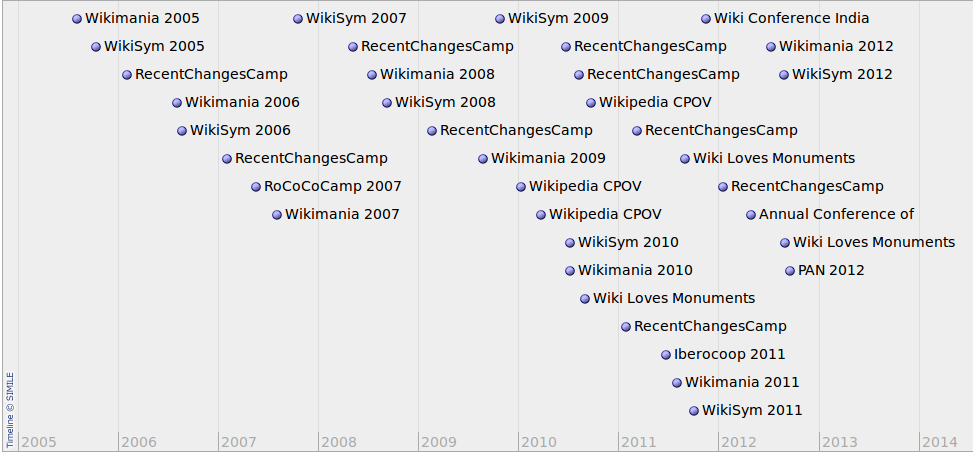
\includegraphics[width=\textwidth]{wptimeline.png} %two-column float
    %\caption{Línea temporal de eventos sobre wikis.}
    \caption{Timeline of events of wikis.}
    \label{fig:wptimeline}
\end{figure*}


\section{Related work}
%Ha habido distintos intentos de recopilar toda la literatura sobre wikis. Se han hecho recopilaciones en páginas personajes y blogs, a través de revisiones de literatura, haciendo uso de gestores de bibliografía, en páginas de Wikipedia y también en servicios como Zotero o CiteULike. A continuación los describimos y evaluamos sus ventajas e inconvenientes y cómo WikiPapers resuelve las carencias de estos enfoques.

There have been several attempts to compile all wiki literature. Among these approaches are compilations in personal websites and blogs, literature reviews, reference management software, Wikipedia pages and online services like Zotero and CiteULike. Following, we describe and assess their advantages and disadvantages and how WikiPapers fixes that.

\subsection{Personal websites and blogs}
%Algunos autores han hecho recopilaciones de literatura en webs personales\footnote{\href{http://www.public.iastate.edu/~CYBERSTACKS/WikiBib.htm}{http://www.public.iastate.edu/~CYBERSTACKS/WikiBib.htm}} y blogs. Un ejemplo bastante completo de este último tipo es SWEETpedia,\footnote{\href{http://www.mkbergman.com/sweetpedia/}{http://www.mkbergman.com/sweetpedia/}} que contiene publicaciones sobre wikis y semántica. Uno de los inconvenientes de este sistema es que el esfuerzo suele recaer sobre una única persona y los metadatos no son fácilmente exportables. En WikiPapers el trabajo se hace colaborativamente y todos los metadatos son fácilmente exportables en diversos formatos.

Some authors have compiled literature in personal websites\footnote{\href{http://www.public.iastate.edu/~CYBERSTACKS/WikiBib.htm}{http://www.public.iastate.edu/~CYBERSTACKS/WikiBib.htm}} and blogs. A very complete example is SWEETpedia,\footnote{\href{http://www.mkbergman.com/sweetpedia/}{http://www.mkbergman.com/sweetpedia/}} which contains publications about wikis and semantic web. This approach has disadvantages: most effort is done by an unique person and metadata is not easily exportable. In WikiPapers, the work is done collaboratively and all metadata is easily exportable in several formats.

\subsection{Reference management software}

\subsubsection{Own servers}
%Se han empleado gestores bibliográficos como WIKINDX\footnote{\href{http://sourceforge.net/projects/wikindx/}{http://sourceforge.net/projects/wikindx/}} creando portales propios como Wikibibliographie ENCYCLEN\footnote{\href{http://wikindx.inrp.fr/biblio_encyclen/}{http://wikindx.inrp.fr/biblio\_encyclen/}} y otros ya desaparecidos, pero como contrapartida decidieron restringir la edición a un círculo de usuarios aprobados. Sin embargo, en WikiPapers pueden participar tanto usuarios registrados como sin registrar.

Reference management software as WIKINDX\footnote{\href{http://sourceforge.net/projects/wikindx/}{http://sourceforge.net/projects/wikindx/}} has been deployed to create portals like Wikibibliographie ENCYCLEN\footnote{\href{http://wikindx.inrp.fr/biblio_encyclen/}{http://wikindx.inrp.fr/biblio\_encyclen/}} and others today disappeared, but registration was mandatory to collaborate. However, anyone can participate in WikiPapers, registration is not needed.

%\href{http://toolserver.org/~voj/bibliography/}{http://toolserver.org/~voj/bibliography/}
%\href{http://wikiindex.org/Wiki_Research_Bibliography}{http://wikiindex.org/Wiki\_Research\_Bibliography}

\subsubsection{Web services and social networks}
%Existen servicios web y redes sociales con recopilaciones de literatura sobre wikis, en Zotero,\footnote{\href{https://www.zotero.org/groups/wikipedia_research}{https://www.zotero.org/groups/wikipedia\_research}} BibSonomy\footnote{\href{http://www.bibsonomy.org/tag/wikipedia}{http://www.bibsonomy.org/tag/wikipedia}} \footnote{\href{http://www.bibsonomy.org/tag/wiki}{http://www.bibsonomy.org/tag/wiki}} y CiteULike.\footnote{\href{http://www.citeulike.org/tag/wikipedia}{http://www.citeulike.org/tag/wikipedia}}\footnote{\href{http://www.citeulike.org/tag/wiki}{http://www.citeulike.org/tag/wiki}}\footnote{\href{http://www.citeulike.org/group/382}{http://www.citeulike.org/group/382}} Este enfoque sí hace uso de una comunidad de usuarios para procesar las publicaciones, pero de nuevo requieren registrarse, y la capacidad de estos servicios para aprovechar los metadatos generando tablas o gráficos es inexistente.

There are wiki literature compilations in web services and social networks, including Zotero,\footnote{\href{https://www.zotero.org/groups/wikipedia_research}{https://www.zotero.org/groups/wikipedia\_research}} BibSonomy\footnote{\href{http://www.bibsonomy.org/tag/wikipedia}{http://www.bibsonomy.org/tag/wikipedia}} \footnote{\href{http://www.bibsonomy.org/tag/wiki}{http://www.bibsonomy.org/tag/wiki}} and CiteULike.\footnote{\href{http://www.citeulike.org/tag/wikipedia}{http://www.citeulike.org/tag/wikipedia}}\footnote{\href{http://www.citeulike.org/tag/wiki}{http://www.citeulike.org/tag/wiki}}\footnote{\href{http://www.citeulike.org/group/382}{http://www.citeulike.org/group/382}} This approach uses a community to process publications, but again registration is mandatory, and there is no capability to generate tables or graphs from the gathered metadata.

\subsection{Compilations in Wikipedia}
%También existen listados de publicaciones y recursos en algunas Wikipedias, como en la versión alemana\footnote{\href{http://de.wikipedia.org/wiki/Wikipedia:Wikipedistik/Bibliographie}{http://de.wikipedia.org/wiki/Wikipedia:Wikipedistik\\ /Bibliographie}} y la inglesa\footnote{\href{http://en.wikipedia.org/wiki/Wikipedia:Academic_studies_of_Wikipedia}{http://en.wikipedia.org/wiki/Wikipedia:Academic\\ \_studies\_of\_Wikipedia}}. El principal inconveniente de este enfoque es que no es posible jugar con los datos dentro del mismo wiki, al estar todo escrito como texto plano, sin enriquecimiento semántico. En WikiPapers todos los metadatos son propiedades semánticas, tanto en las llamadas \emph{infoboxes} (tablas) como en el cuerpo del artículo.

Also, there are lists of publications and resources in some Wikipedias, as the German\footnote{\href{http://de.wikipedia.org/wiki/Wikipedia:Wikipedistik/Bibliographie}{http://de.wikipedia.org/wiki/Wikipedia:Wikipedistik\\ /Bibliographie}} and English ones\footnote{\href{http://en.wikipedia.org/wiki/Wikipedia:Academic_studies_of_Wikipedia}{http://en.wikipedia.org/wiki/Wikipedia:Academic\\ \_studies\_of\_Wikipedia}}. The main drawback is that you can't reuse and explore the data because it is just plain text without semantic enrichment. In wikiPapers all metadata are linked to semantic properties, including \emph{infoboxes} and the article body text.

\subsection{Literature reviews}
%Finalmente, se han realizado varias revisiones de literatura con diferente grado de exhaustividad. La primera de ellas ~\citep{voss2005} se hizo en un momento en el que las publicaciones eran escasas, pero ya se podía ver una tendencia de publicación creciente y la presencia de muchas preguntas por responder. Un año más tarde ~\citep{ayers2006} vuelve a hacer un repaso a la literatura existente y enumera aquellas áreas que han recibido interés: historiales, páginas de discusión, contenido de los artículos, políticas del sitio, citas a artículos, encuestas a usuarios y listas de correo.

Finalmente, se han realizado varias revisiones de literatura con diferente grado de exhaustividad. La primera de ellas ~\citep{voss2005} se hizo en un momento en el que las publicaciones eran escasas, pero ya se podía ver una tendencia de publicación creciente y la presencia de muchas preguntas por responder. Un año más tarde ~\citep{ayers2006} vuelve a hacer un repaso a la literatura existente y enumera aquellas áreas que han recibido interés: historiales, páginas de discusión, contenido de los artículos, políticas del sitio, citas a artículos, encuestas a usuarios y listas de correo.

No sería hasta 3 años después cuando \cite{okoli2009b} presentan una propuesta de protocolo para hacer un mapeo sistemático de la literatura sobre Wikipedia, indicando la existencia de más de 1.000 publicaciones y ese mismo año \cite{okoli2009} analiza el estado del arte. Dos años más tarde, \cite{nielsen2011} hace la mayor revisión de literatura en un documento de más de 50 páginas, en progreso e inacabado, que incluye 300 referencias a publicaciones y reincide en la existencia de 1.000 publicaciones sobre el tema.

\cite{martin2011} hace primero un repaso técnico a la estructura de la base de datos (páginas, usuarios, texto), luego se centra en las áreas de calidad y acaba con unas consideraciones filosóficas.

\cite{okoli2012} (the WikiLit review) es una revisión de literatura sobre Wikipedia exclusivamente, unas 450 publicaciones. Reutilizan las plantillas, formularios, semántica y estructura de WikiPapers. Pretenden incorporar sus resultados a WikiPapers en algún momento.

La revisión más reciente \cite{jullien2012} hace un repaso por las motivaciones para contribuir, roles, estructura, la vida de un artículo, calidad, experiencia de usuario y accesibilidad, entre otros.

Uno de los inconvenientes de estas revisiones de literatura es que quedan rápidamente desactualizadas debido al ritmo con el que aparecen nuevas publicaciones. WikiPapers es actualizado continuamente por su comunidad de voluntarios.

\section{WikiPapers}
WikiPapers\footnote{\href{http://wikipapers.referata.com}{http://wikipapers.referata.com}} fue lanzado en abril de 2011 (Figura~\ref{fig:wpfull}). Haciendo uso de MediaWiki y su extensión semántica, recopila de manera colaborativa información acerca de toda la literatura sobre wikis, así como de herramientas y \emph{datasets} relacionados. No hace falta estar registrado para participar, aunque es recomendable.

WikiPapers agrupa todas las ventajas de los sistemas mencionados anteriormente y soluciona sus inconvenientes. Permite hacer listados específicos de publicaciones, similares a SWEETpedia: por poner un ejemplo, existe uno de revisiones de literatura.\footnote{\href{http://wikipapers.referata.com/wiki/List_of_literature_reviews}{http://wikipapers.referata.com/wiki/List\_of\\ \_literature\_reviews}} Funciona como un gestor bibliográfico, al almacenar los metadatos de las publicaciones y permitir hacer búsquedas, filtrarlos o exportarlos, individualmente o en conjunto. También facilita que grupos de usuarios se comuniquen a través de las páginas de discusión y compartan información sobre publicaciones de su interés, funcionando como una red social. Por otro lado, el espacio de discusión debajo de cada página posibilita a los lectores hacer valoraciones de los artículos. Y al ser un wiki, puede ser constantemente mejorado, evitando quedar desactualizado debido al rápido ritmo de publicación.

Desde un punto de vista más estadístico, es posible generar gráficas y tablas a partir de los metadatos disponibles en WikiPapers, aprovechando así la capacidad que ofrece la semántica. Gráficos de barras, circulares o líneas temporales están presentes y facilitan la visualización y comprensión de la información. También existe la posibilidad de incrustar diapositivas (SlideShare) y vídeos (YouTube, Vimeo).

Finalmente, el wiki y sus historiales están disponibles tanto para su descarga en XML y accesible a través de la API de MediaWiki. Esto impide que todo el trabajo se pierda, como ha sucedido en otros proyectos que quedaron inactivos y finalmente desaparecieron.

\begin{figure}[htb]
\centering
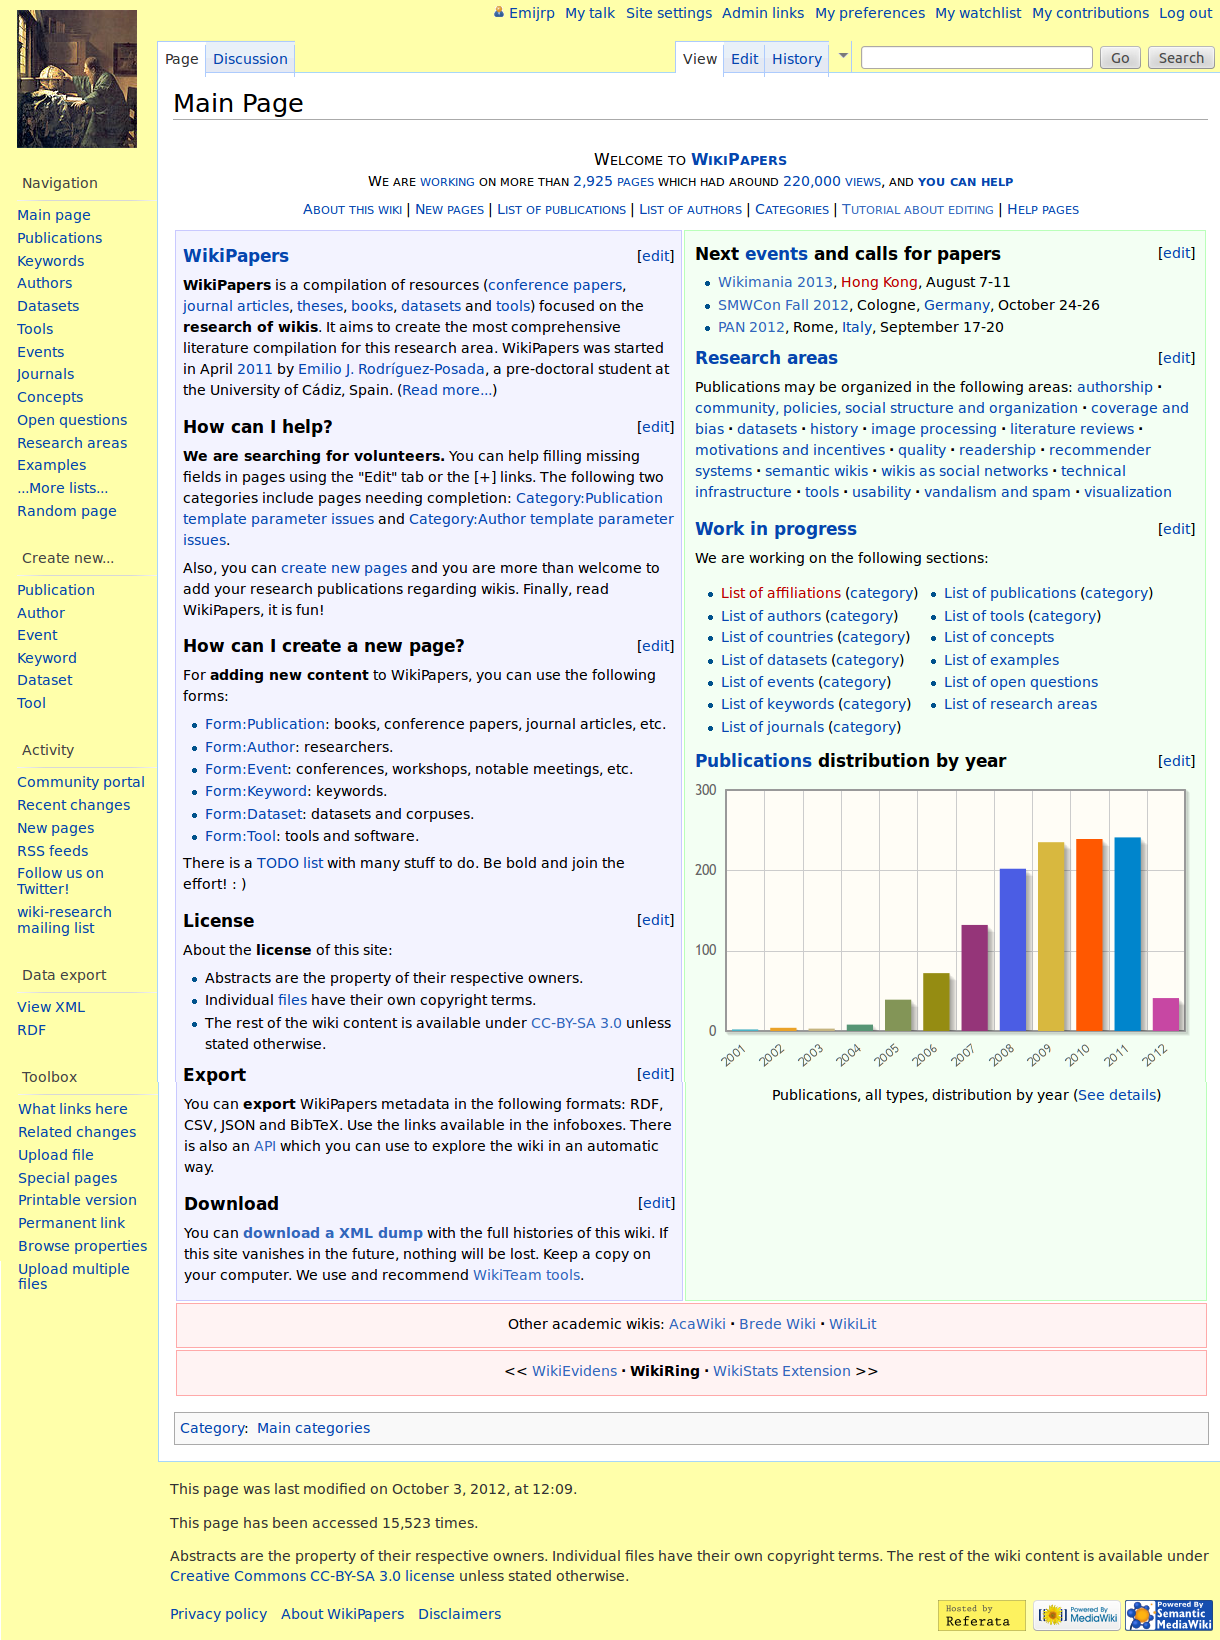
\includegraphics[width=0.49\textwidth]{wpfull.png}
\caption{WikiPapers mainpage.}
\label{fig:wpfull}
\end{figure}

\subsection{Publications}
En WikiPapers cada publicación dispone de una página en la que se detallan todos sus metadatos (título, autores, palabras clave, año, revista o congreso, DOI, idioma, licencia, enlaces al fichero y motores de búsqueda), el abstract, las referencias que incluye, las citas que recibe y un espacio de discusión. Los metadatos sirven para hacer búsquedas y filtrar. A noviembre de 2012 ya se dispone de más de 1.700 publicaciones,\footnote{\href{http://wikipapers.referata.com/wiki/List_of_publications}{http://wikipapers.referata.com/wiki/List\_of\_publications}} incluyendo artículos de revistas y congresos, tesis y libros. Todos los metadatos se pueden exportar en los formatos BibTeX, RDF, CSV y JSON.

\subsection{Keywords}
Existe un listado de todas las palabras clave\footnote{\href{http://wikipapers.referata.com/wiki/List_of_keywords}{http://wikipapers.referata.com/wiki/List\_of\_keywords}} presentes en los artículos y cada una de ellas cuenta con varios términos relacionados, lo que permite navegar entre ellas. Las más frecuentes son: Wikipedia, wiki, semantic wiki, web 2.0, collaboration, evaluation, collaborative learning, knowledge management, MediaWiki, motivation, data mining y conflict. 

\subsection{Authors}
Para cada autor hay una ficha que incluye su nombre, afiliación, país, índice de coautores, página web, estadísticas sobre número de publicaciones y citas, y por supuesto un listado de publicaciones, \emph{datasets} y herramientas de su creación. Ya están listados unos 1.000 autores.\footnote{\href{http://wikipapers.referata.com/wiki/List_of_authors}{http://wikipapers.referata.com/wiki/List\_of\_authors}}

\subsection{Datasets}
Un listado de \emph{datasets}\footnote{\href{http://wikipapers.referata.com/wiki/List_of_datasets}{http://wikipapers.referata.com/wiki/List\_of\_datasets}} permite observar la gran cantidad de datos sobre comunidades wiki disponibles para analizar. Existen \emph{datasets} sobre vandalismo, texto wiki enriquecido con semántica, datos extraidos de \emph{infoboxes}, \emph{logs} anonimizados de visitas, mensajes de listas de correo y por supuesto los historiales de Wikipedia.

A este respecto, el proyecto WikiTeam\footnote{\href{http://code.google.com/p/wikiteam/}{http://code.google.com/p/wikiteam/}} está compilando una gran cantidad de datos sobre comunidades wiki, que se cifra ya en 4.500 \emph{dumps}.

\subsection{Tools}
Se está construyendo un listado de herramientas\footnote{\href{http://wikipapers.referata.com/wiki/List_of_tools}{http://wikipapers.referata.com/wiki/List\_of\_tools}} que se han desarrollado a la hora de investigar sobre wikis y para proponer soluciones a ciertos problemas. Entre ellas se incluyen:

\begin{itemize}
\item \textbf{Anti-vandalismo:} AVBOT, Clue Bot, CryptoDerk's Vandal Fighter, Huggle, Igloo, STiki, Salebot, Twinkle, Vandal Fighter, VandalProof, VandalSniper.
\item \textbf{Estadística y visualización:} HistoryFlow, StatMediaWiki, Wiki Explorator, Wiki Trip, WikiEvidens, WikiTrust.
\item \textbf{Frameworks:} Java Wikipedia Library, Perlwikipedia, pywikipedia.
\item \textbf{Lenguaje:} Manypedia, Wikokit, Zawilinski.
\item \textbf{Preservación:} WikiTeam tools.
\item \textbf{Procesamiento de datos:} DiffDB, Ikiwiki, Infobox2rdf, Wiki Edit History Analyzer, Wikihadoop, Wikipedia Miner.
\end{itemize}

La lista no es exhaustiva y está en continuo crecimiento.

\subsection{And more...}
También se está recopilando información sobre revistas, congresos, eventos, conceptos, ejemplos de análisis, preguntas abiertas, encuestas, motores wiki, wikifarms y más. WikiPapers, además de todo lo comentado anteriormente, sirve para que investigadores de wikis hagan comunidad y establezcan conexiones para futuras investigaciones.

\section{Conclusions and future work}
El estudio de los wikis es un campo emergente y prolífico. Hasta ahora la recopilación de toda la literatura sobre wikis se había abordado de distintas formas. Se han utilizado webs personales, blogs, gestores bibliográficos, servicios web, redes sociales, pero cada uno tiene sus ventajas e inconvenientes. Ninguno de ellos ha conseguido ser exhaustivo y permanecer actualizado con el paso del tiempo.

En este artículo hemos presentado WikiPapers, un proyecto colaborativo para recopilar toda la literatura sobre wikis. Se hace uso de MediaWiki y su extensión semántica, ambos conocidos por los investigadores de este campo.

En noviembre de 2012 cuenta ya con información de más de 1.700 publicaciones, además de documentación sobre herramientas y \emph{datasets} relacionados. Los metadatos son exportables en los formatos BibTeX, RDF, CSV y JSON. Los historiales completos del wiki están disponibles para descarga y facilitar su preservación. 

WikiPapers es una comunidad abierta a la participación. Estamos recopilando colaborativamente toda la literatura sobre wikis... ¡en un wiki!

%\bibliographystyle{wink}
\bibliographystyle{hunsrtnat}
\bibliography{wikipapers-2012}

\section*{Acknowledgements}

Me gustaría agradecer a Izaskun Mallona el trabajo que se ha tomado revisando este artículo y su ayuda en general. Y a los colaboradores de WikiPapers, que han dedicado su tiempo a mejorar los contenidos del sitio.

\section*{License}
This work is licensed under a \href{http://creativecommons.org/licenses/by-sa/3.0/}{Creative Commons Attribution-ShareAlike 3.0 Unported}.

\end{document}
